\section{Object Detection}
\label{sec:ObjectDetection}

Since the topic of this thesis concerns the task of \emph{visual} object tracking, an indispensable step in the processing pipeline will unquestionably be object detection. Here we give an overview of various types of image inference to highlight the importance of object detection. The general task of image inference comes in three types, where each builds upon the previous one. The dependency chain is the following: \emph{object classification} $\to$ \emph{object detection} $\to$ \emph{image segmentation}.

Object detection comes in various flavors discussed in the following sections. From a holistic point of view, there are \emph{fast} object detectors, such as the most prominent one, \gls{yolo}~\cite{redmon2016yolo} (\sectionstr{}~\ref{ssec:YouLookOnlyOnce}), or \gls{ssd}~\cite{liu2016ssd}. Here, we use the term \emph{fast} to denote that the detector can operate on high \gls{fps}. This comes at a cost of relatively lower accuracy, though, as compared to \emph{slower} but more accurate approaches based on region proposals, such as various versions of \fasterrcnn{} (section \ref{ssec:FasterRCNN}).

Historically speaking, object detection in its early stages of development depended on feature engineering followed by some shallow machine learning model (e.g. \gls{svm}~\cite{cortes1995support}) to classify the proposed object. Feature extraction was achieved using approaches such as \gls{sift}~\cite{lowel1999objrecognition}, an algorithm capable of producing description of local features in images. Another eminent approach was \gls{hog}~\cite{mcconnell1986osti}, equally used for feature extraction by taking advantage of a change in orientation of gradients in localized portions of the image and subsequently counting occurrences of various orientations. But, as we stated, robust object detection is what our task demands, and the goal of getting the top performance is unattainable without deep learning-based object detection, the principal topic of this section.

Object detection is by its very nature a difficult task, because the number of objects is unknown in advance, which means, that the number of outputs of the model is variable. A plethora of attempts have been proposed to evade this inherent shortage of standard neural networks. An obvious solution is to only produce a constant number of \glspl{bbox}, as utilized by \gls{ssd} and \gls{yolo}, for instance. But methods based on region proposals try to circumvent the obstacle of having to predict only a fixed set of \glspl{bbox}. Other differences between object detectors stem from the architecture itself, whether the training is an end-to-end pipeline or the model consists of various parts. Fully convolutional architectures are also becoming more prevalent and the latest results are promising~\cite{tian2019fcos}. We will also review fully convolutional trackers in great detail in section \ref{ssec:FullyConvolutionalTracking}.

% ##############################################################################
\subsection{Non-Maximum Suppression}
\label{ssec:NonMaximumSuppression}

Before we dive into the description of the detection itself, we first introduce a general post-processing approach for test phase inference of an object detector. Object detectors have hugely profited from the so-called end-to-end learning paradigm in which object proposals, features, and the classifier become part of one neural network model~\cite{hosang2017learningnms}. A proposal, in this setting, is nothing but a region containing a potential object of interest. However, the number of proposals may grow considerably, outnumbering the real count of present objects of interest. Moreover, these proposals may have a large overlapping region as measured by \gls{iou} ( \sectionstr{}~\ref{eq:IntersectionOverUnion}), rendering most of them useless in terms of conveying new information, as the majority could cover pretty much the same region. To filter such proposals and extract only the relevant ones, the \gls{nms} algorithm introduced below is used (see \figstr{}~\ref{fig:NonMaximumSuppression}). The central idea is to iteratively select only region proposals the \gls{iou} of which is below a specific threshold, i.e. the area they share does not exceed a particular value.

For a more formal description, let $\mset{B} = \cbrackets{\vect{b}_1, \vect{b}_2, \dots, \vect{b}_n}$ be a set of $n$ region proposals described by $n$ \glspl{bbox}. Scores for each detection are contained in a set $\mset{S} = \cbrackets{s_1, s_2, \dots, s_n}$, where $s_i$ denotes a detection score for the $i$-th box, $\vect{b_i}$. Let $\lambda$, such that $0 \leq \lambda < 1$, denote a threshold for the maximum allowed portion of the overlap between regions. $\mset{B}_{nms}$ is the set of filtered proposal instances from the set $\mset{B}$ produced using the \gls{nms} algorithm below (inspired by~\cite{bodla2017softnms}):

\begin{algorithmic}[1]
    \Function{NMS}{$\mset{B}$, $\mset{S}$, $\lambda$}

    \State $\mset{B}_{nms}$ $\gets$ $\emptyset$
    \Comment{initialize the output (filtered) set of region proposals}

    \While {$\mset{B} \neq \emptyset$}
    \Comment{loop until all the proposals are processed}

    \State $m \gets \underset{i \in \cbrackets{1, 2, \dots, \msetsize{S}}}{\argmax{}} \mset{S}$
    \Comment{find an index of a proposal with the highest score}

    \State $\mset{B} \gets \mset{B} - \vect{b}_m$, $\mset{S} \gets \mset{S} - s_m$
    \Comment{remove the proposal}

    \State $\mset{B}_{nms} \gets \mset{B}_{nms} \cup \vect{b_m}$
    \Comment{save the proposal with the highest score}

    \For{$i \gets 1$ to $\msetsize{B}$}
    \Comment{iterate through remaining proposals}

    \If{\Call{iou}{$\vect{b}_m$, $\vect{b}_i$} $\geq \lambda$}
    \Comment{\gls{iou} (equation~\ref{eq:IntersectionOverUnion}) exceeds the threshold}

    \State $\mset{B} \gets \mset{B} - \vect{b}_i$, $\mset{S} \gets \mset{S} - s_i$
    \Comment{remove the proposal}
    \EndIf
    \EndFor
    \EndWhile

    \State \Return $\mset{B}_{nms}$
    \EndFunction
\end{algorithmic}

\begin{figure}[t]
    \centerline{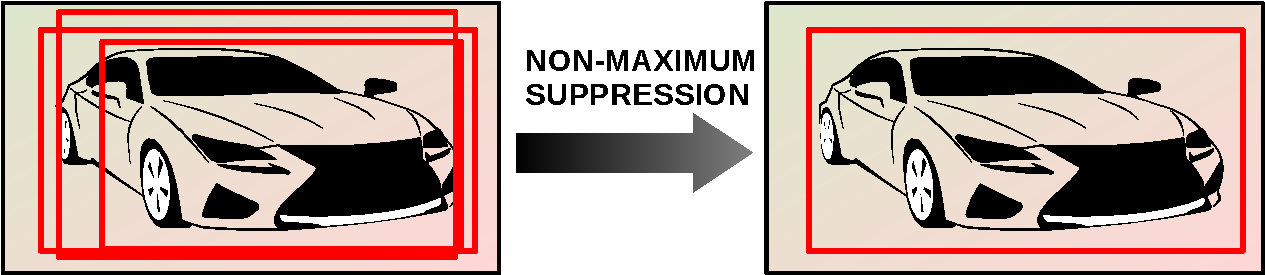
\includegraphics[width=0.6\linewidth]{figures/theoretical_foundations/non_maximum_suppression.pdf}}
    \caption[\Gls{nms} visualization]{An illustration of a potential effect of the \gls{nms} algorithm on \glspl{bbox}. Multiple proposals (left) are filtered so that only the ones with the highest detection score (right) remain while satisfying the condition that the overlap does not exceed a specific threshold.}
    \label{fig:NonMaximumSuppression}
\end{figure}

% ##############################################################################
\subsection{YOLO}
\label{ssec:YouLookOnlyOnce}

\Gls{yolo} is a very popular single-stage object detector thanks to its ability to run in real-time and yet be very accurate. Its speed is primarily a consequence that \emph{it looks only once} at a given input image. Compared to region proposal-based approaches, where each object proposal has to be classified separately, resulting in multiple inferences by a potentially huge neural network model, the authors of \gls{yolo} devised a \gls{cnn} model capable of performing extraction of region proposals as well as classification in a single run~\cite{redmon2016yolo}. Besides, the backbone \gls{cnn} model responsible for handling the visual input processes an entire image during the training and test time, allowing the implicit inclusion of contextual information about classes together with their visual representation. During the testing phase, after the single forward propagation through the neural network is executed, the \gls{nms} algorithm is employed to filter predictions to make sure that each object instance is detected just once. Since the initial introduction of this approach~\cite{redmon2016yolo}, multiple updates have been brought forward, either from the main author himself~\cite{redmon2017yolo9000, redmon2018yolov3}, or from other researchers~\cite{wang2020yolov4, wong2019yolonano}. Such an interest supports the assertion that \gls{yolo} has great potential for further research as well as real-world applications. Despite its populality, for our experiments, we employed the paragon of two-stage object detection, discussed next.

% ##############################################################################
\subsection{Faster R-CNN}
\label{ssec:FasterRCNN}

The \fasterrcnn{}~\cite{ren2017fasterrcnn} is the most prominent \emph{two-stage} object detector. The first stage consists of generating region proposals using the \gls{rpn} (see \figstr{}~\ref{fig:FasterRCNNRPN}), where the input image is processed by a feature extractor~\cite{huang2017speedacctradeoff}. These class-agnostic proposals, a set of rectangular \glspl{bbox}, are produced from an input of arbitrary size (allowed by the fact that this process is modeled by a fully convolutional network) (see \figstr{}~\ref{fig:FasterRCNNMetaArch} and \figstr~\ref{fig:FasterRCNNPipeline}).

As far as the second stage is concerned, the proposed regions (usually $300$) serve as a basis for subsequent cropping of features from the same intermediate feature map which are then fed to the remaining feature extractor to predict the class. Based on this class prediction, the proposed box is further refined. The name for this stage is \emph{box classifier}.

\begin{figure}[t]
    \centerline{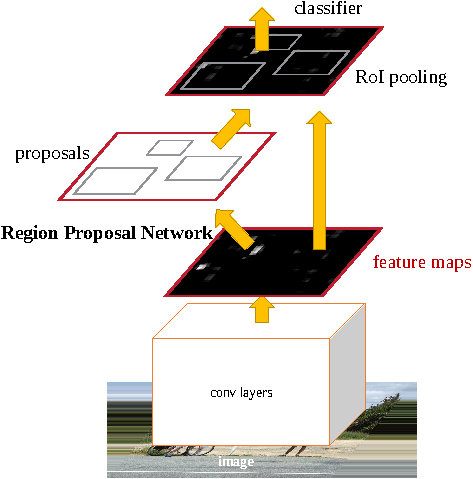
\includegraphics[width=0.5\linewidth]{figures/theoretical_foundations/faster_rcnn_rpn_module.pdf}}
    \caption[\fasterrcnn{} with the \gls{rpn}]{The \fasterrcnn{} is built as a unified network for object detection, with its \gls{rpn} module serving the purpose of an \emph{attention}. \externalsrc{\cite{ren2017fasterrcnn}}}
    \label{fig:FasterRCNNRPN}
\end{figure}

\begin{figure}[t]
    \centerline{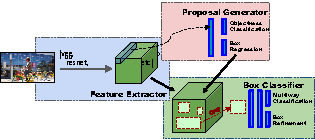
\includegraphics[width=0.65\linewidth]{figures/theoretical_foundations/faster_rcnn_metaarchitecture.pdf}}
    \caption[\fasterrcnn{} meta-architecture]{A meta-architecture of the \fasterrcnn{} model. \externalsrc{\cite{huang2017speedacctradeoff}}}
    \label{fig:FasterRCNNMetaArch}
\end{figure}

As the endeavor is to diminish unnecessary computations, the proposals are not cropped explicitly from the input image, and then processed by the feature extractor. Nevertheless, there is a part of the computation that has to be executed once per each proposed region, so the performance depends on the number of regions generated by the \gls{rpn}.

\begin{figure}[t]
    \centerline{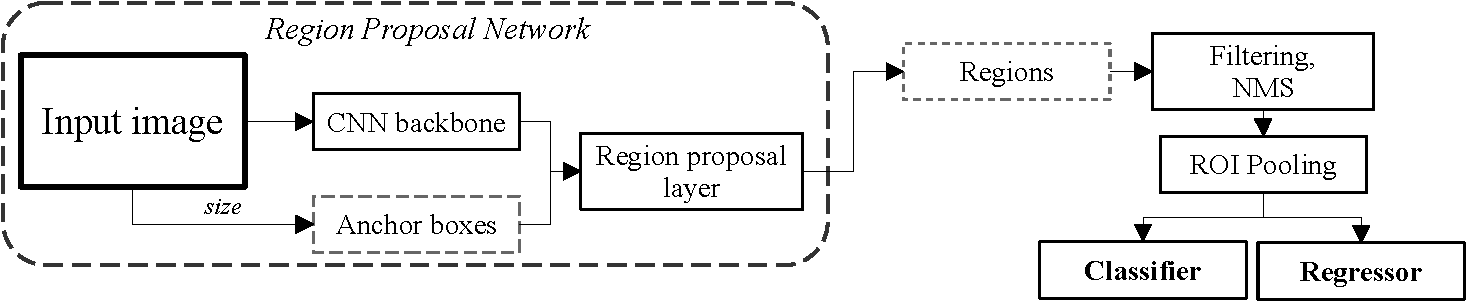
\includegraphics[width=\linewidth]{figures/theoretical_foundations/fastercnn_diagram.pdf}}
    \caption[\fasterrcnn{} processing diagram]{A conceptual diagram of the \fasterrcnn{} model demonstrating the information pipeline when processing an input image.}
    \label{fig:FasterRCNNPipeline}
\end{figure}

This architecture is especially important for this treatise as it formed a base object detector for the multi-object tracker with which we conducted the majority of our object tracking research.
